\documentclass{beamer}
\usepackage[orientation=landscape, size=a0, scale=1.4]{beamerposter}
\usepackage[absolute,overlay]{textpos}
\usepackage{multicol}
\usepackage{graphics}
\usepackage{url, enumitem}
\usepackage{amsfonts}
\usepackage{listings}
\usepackage{graphicx}
\usepackage{bm}
\usepackage{tikz}
\usetikzlibrary{fit,positioning}
  \usetheme{CambridgeUS}
    \title[Designator]{Designator}
    \addtobeamertemplate{frametitle}{\vskip0.6ex}{}
\usepackage{scrextend}
\changefontsizes{29pt}
\begin{document}

%\begin{block}{\centering \Huge {Title Goes Here}}
%\end{block}
\begin{frame}{\centerline{\Huge Designator - Using Ducks to understand Web Design}}
\begin{textblock}{5}(.15,.85)
\begin{block}{Introduction}
Over the past decade, aesthetics have gained a lot of importance in the decisions companies
make in how they design websites, and user experience is at the core of this trend.  In this paper, we develop a way to automate this process by generating color suggestions based on what we call the "Ugly Duckling" problem: essentially recommending what popular similar websites contain that the input website does not yet have. Using Ugly Duckling, we got results that are consistently better than color recommenders based on more classical techniques such as Naive Bayes, SVM, and Random Forest classification. It is not immediately clear, however, how to find "similar websites." Especially when the website dabatase is large, diffing a screenshot or even the color histogram of a given input website against thousands or millions of other websites can prove to be a daunting task. This paper applies different sorts of unsupervised clustering including KMeans and Affinity Propagation to solve this problem. Once the websites are clustered, the system can place
an input website into a cluster. Diffing the input against all websites in a cluster can be
done much faster than within the whole database,anybody faanybody fa and the system will only have to conside
recommendations that are relevant to that specific cluster.

Note that this type of recommendation is not limited to web design and can theoretically be used for other visual medias such as art.
\end{block}

\begin{block}{Data}
Our data consists of the 5000 most popular websites on the web drawn from the Alexa database, whose screenshots we got using PhantomJS. To keep the data clean, we purged all uninteresting websites that have only 2 or less colors. For feature vectors, we used both ~7000 dimensional RGB arrays and $D=$~17000 dimensional binned histograms. The binned histograms are color histograms where we place color values into bins of size 10, so that we consider the existence of exactly $D$ colors as opposed to the usual 255 * 255 * 255 which is too large.
\end{block}

\begin{block}{Problem and Error Measuring}
Website data is completely unlabeled and it is not immediately clear what a "good" color recommendation would be. To address this issue, we remove a color $c$ from each website in the test set and ask our system to try to recommend it back. In this framework, recommendation becomes a classification problem that tries to infer $c$ out of ~17000 different possible colors, so throughout the paper we consider both the classification accuracy $\tau$ as a percentage (greater is better, doesn't take into account how distant the colors are) and the mean color recommendation error $\delta$ (lower is better, takes into account how distant the colors are).
$$\tau_Y = \frac{\text{Correct}}{\text{Total}} = \frac{\sum_n I[r_n = c_n]}{n}$$
$$\delta_Y = \sum_n |r_n - c_n|$$
\end{block}

\begin{block}{Model of the Problem}
Consider our problem represented by the following graphical model
\begin{figure}
\centering
\begin{tikzpicture}
\tikzstyle{main}=[circle, minimum size = 10mm, thick, draw =black!80, node distance = 16mm]
\tikzstyle{connect}=[-latex, thick]
\tikzstyle{box}=[rectangle, draw=black!100]
\node[main, fill = white!100] (Color) []{$C$ };
\node[main] (Web) [right=of Color] {$W$};
\node[main,fill={rgb:red,243;green,243;blue,243}] (WebLessColor) [above=of Web, yshift=15mm, xshift=-10mm] {$W_{c}$};
  \path 
  	(Web) edge [connect] (Color)
  	(Color) edge [connect] (WebLessColor)
  	(Web) edge [connect] (WebLessColor);
\end{tikzpicture}
\end{figure}
Where $W$ is the initial (unobserved) website, $C$ is the removed color that we wish to predict, and $W_c$ is the website
that we observe, after having $C$ removed. In our case, $C$ is chosen uniformly from $W$ (except we never let $C$ be a
background color, i.e. a color that takes up more than 40\% of the page, because those colors are uninteresting as
recommendations).
\end{block}


\begin{block}{Approach - The Ugly Duckling Algorithm}
Given the model above, it makes sense to try to predict the color $C$ by looking at websites similar to $W_c$, hoping
that they might contain $C$ is as well. From this intuition we developed theUgly Duckling recommendation algorithm: given some input website $x$, we take a list of similar websites $Y$ and find the color not present in $x$ that appears most consistently in $Y$.
$$r = \text{argmax}_{d} \text{mean}(Y_d) $$
where $Y_d$ is the $d$-th color of a website in $Y$. We also explored with similar formulas that also take variance into account such as
$$r = \text{argmax}_{d} \frac{E\left[Y_d\right]}{\text{var}(Y_d)} $$
but found the first one to be the most reliable.

Now we are left with the problem of finding websites that are "similar" to our input. Our first idea was to use
clustering algorithms such as KMeans and Affinity Propagation. We used the sk-learn version of KMeans and implemented
Affinity Propagation ourselves in Python. The results of these algorithms on our data set can be seen in the following
section.
\end{block}


\end{textblock}

\begin{textblock}{5}(5.5, .85)

\begin{block}{K-Means using Images}
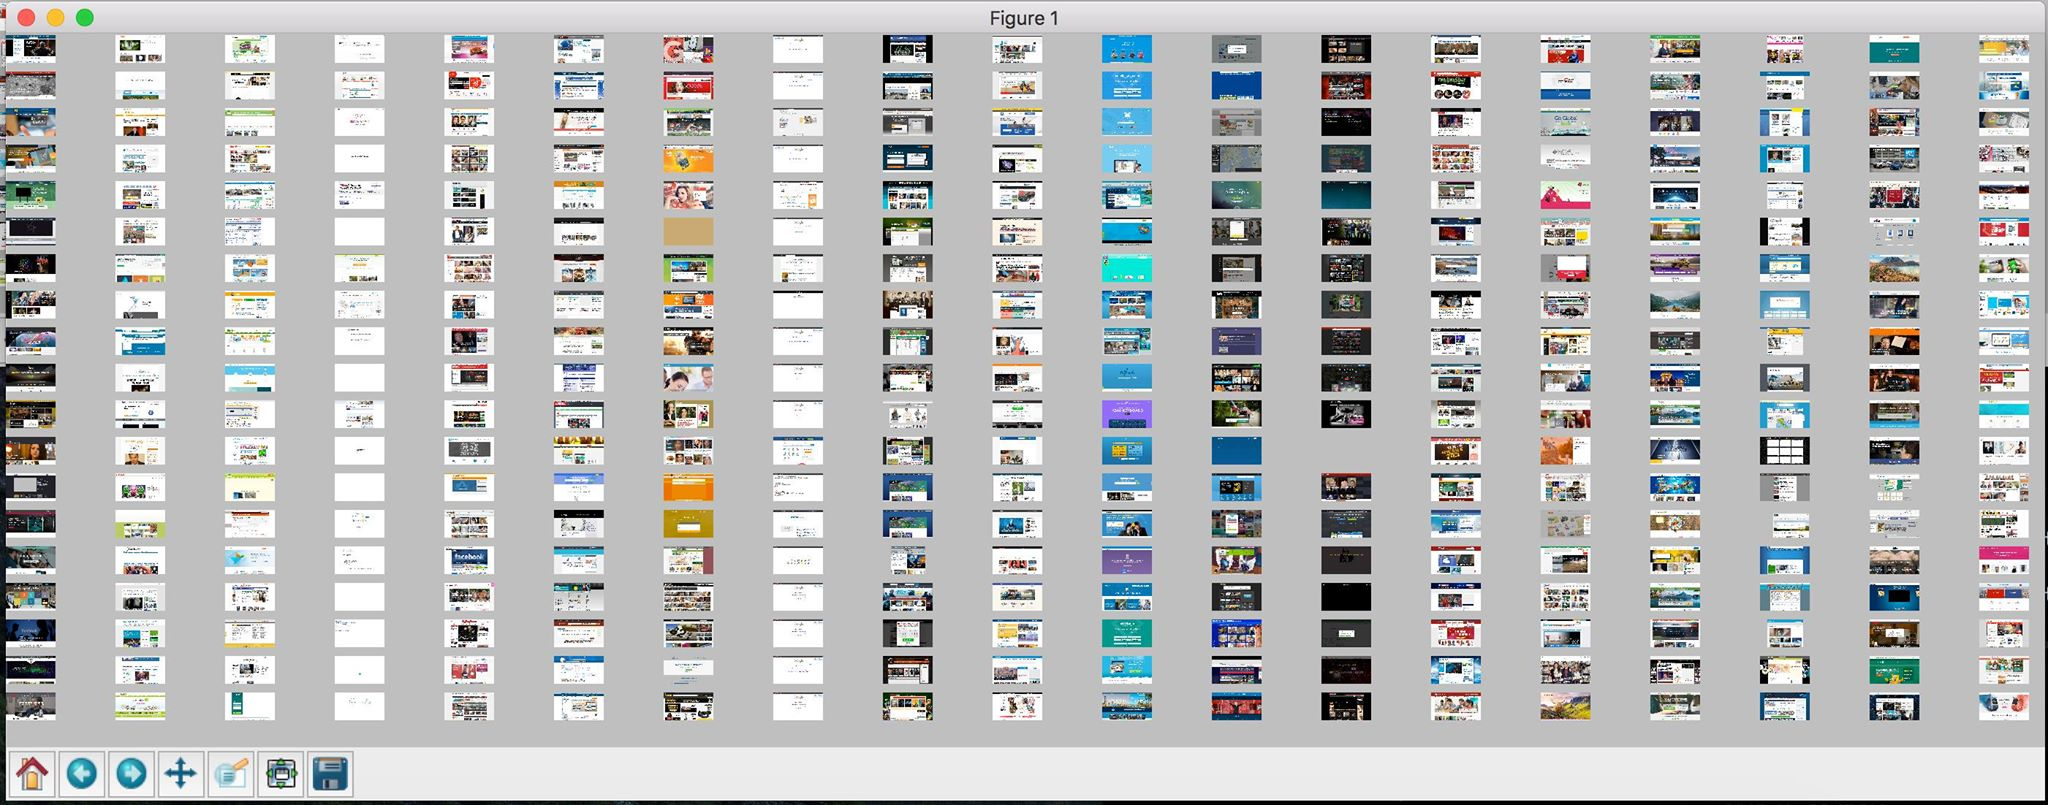
\includegraphics[scale=.45]{imgkmeans.png}
\end{block}
\begin{block}{Affinity Propogation using Image}
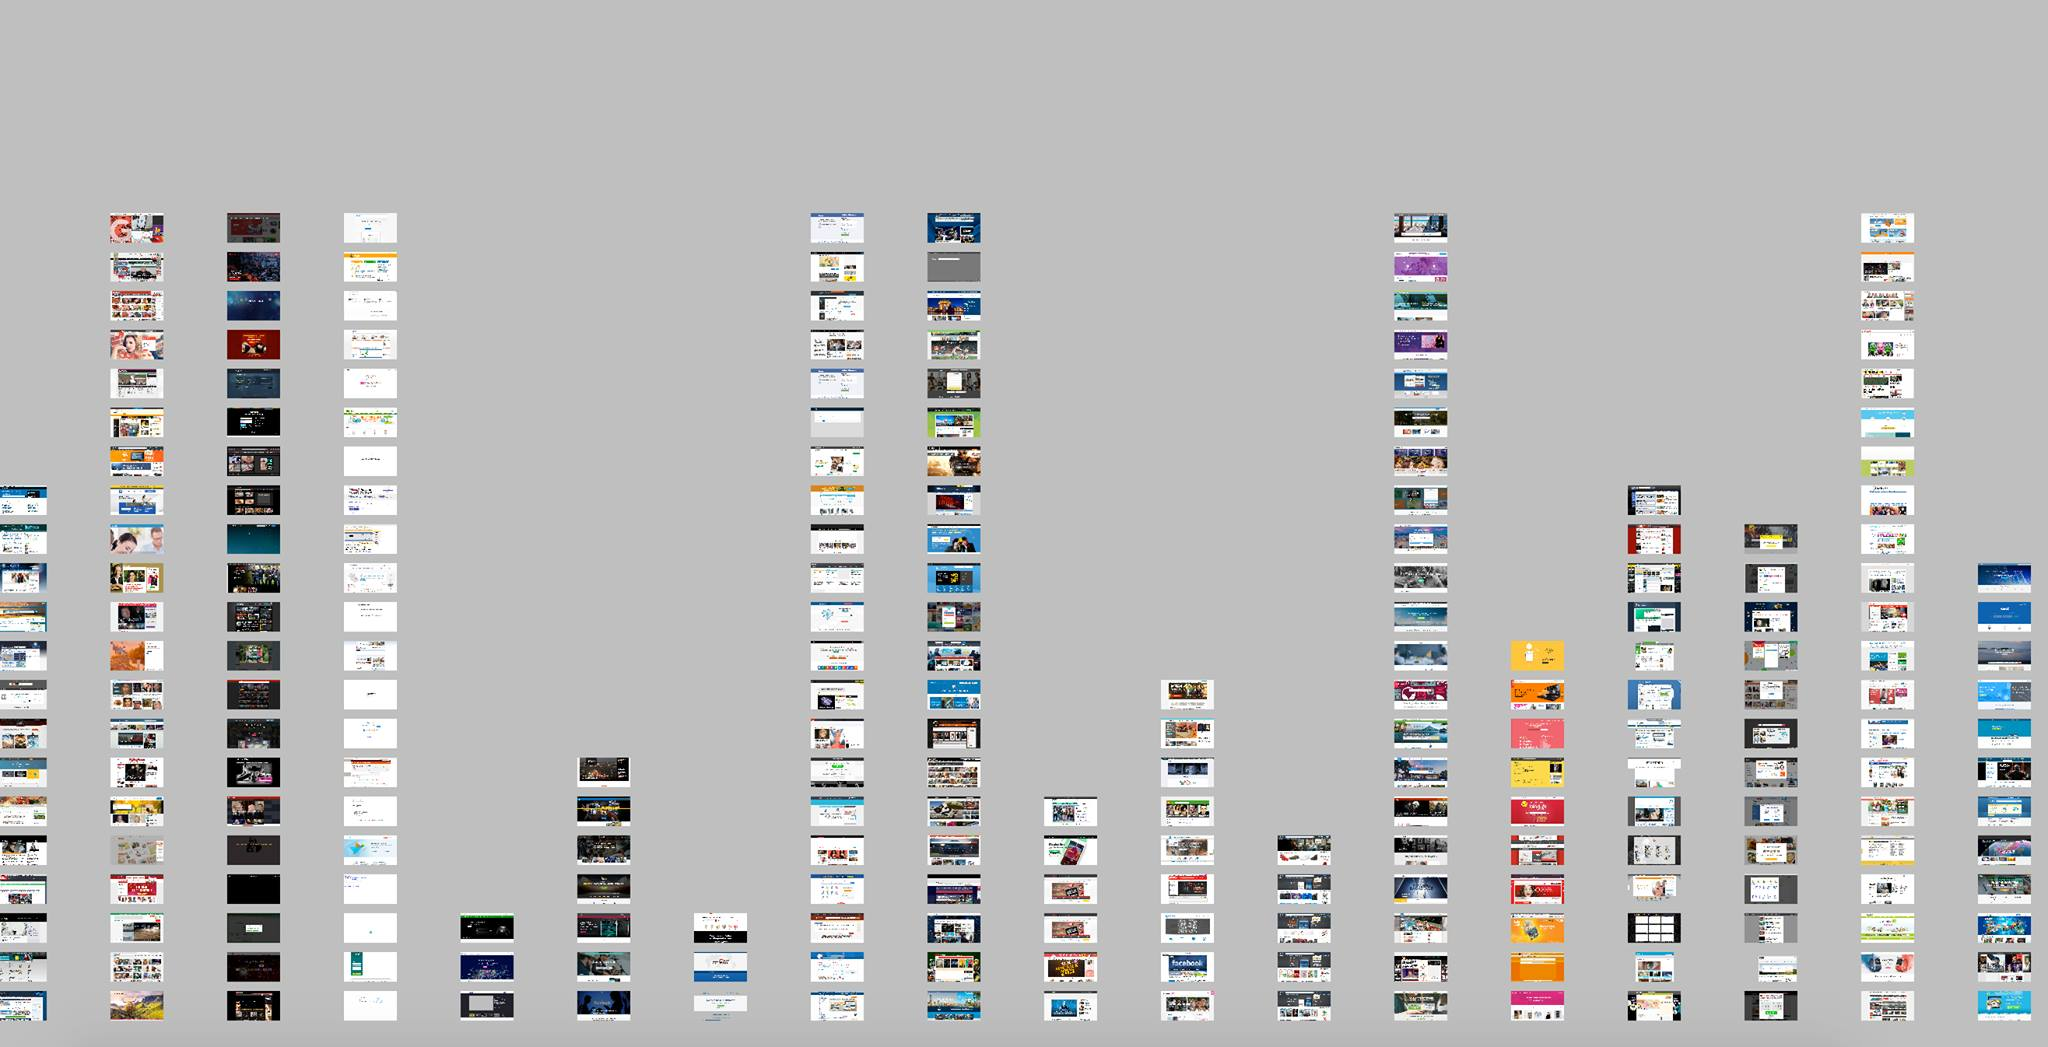
\includegraphics[scale=.45]{affPropImg.jpg}
\end{block}
\begin{block}{Affinity Propogation Model}
\begin{figure}
\centering
\begin{tikzpicture}
\tikzstyle{main}=[circle, minimum size = 10mm, thick, draw =black!80, node distance = 16mm]
\tikzstyle{connect}=[-latex, thick]
\tikzstyle{box}=[rectangle, draw=black!100]
\node[main, fill = white!100] (d)  {$d_i$};
\node[main, fill = white!100] (e) [above= of d] {$e_j$};
\node[main, fill = white!100] (s) [below= of d] {$s_i$};
  \path (e) edge [connect] (d)
  	(d) edge [connect] (e)
  	(s) edge [connect] (d);
  \node[rectangle, inner sep=4mm, draw=black!100, fit = (s)(d), label=below right:N] {};
  \node[rectangle, inner sep=4mm, draw=black!100, fit = (e), label=below right:N] {};
\end{tikzpicture}
\end{figure}

Where an arrow from a $d_i$ to a $e_j$ represents how ``responsible'' a given data point is for another (i.e., how good of a choice it would be to choose $e$ as an exemplar for $d$), an arrow from $e_j$ to $d_i$ asks how ``available'' a data point is to pick $e_j$ as an exemplar for $d_i$, taking into account other $d$'s preferences for $e$ as an exemplar, and $s_i$ is a prior over how similar two points can be. This is calculated by first calculating the euclidian distance between this website and all other websites, and then taking the median value of this set.
\end{block}
\begin{block}{Recommendations}
\includegraphics[scale=.5]{fullDuck.jpg}
\includegraphics[scale=.4975]{randomForest.jpg}
\includegraphics[scale=.35]{affProp.jpg}


\end{block}
\end{textblock}

\begin{textblock}{5}(10.75, .85)
\begin{block}{Intermediate Solutions - The Life of a Duck}
We initially started with a naive recommendation scheme that considers only the image in the data set that is closest to our input (by diffing
histograms). From there, we recommend adding the color that would bring the two images the
closest.

Then we moved on to the Ugly Duckling algorithm using clusters. Given an input website, we'd first place it into a
cluster and consider that cluster the set of similar websites where we'd try to find the color $C$. Initially we used K-means and
Affinity Propagation for clustering, which already improved our classification rate by over 50 times.
\end{block}

\begin{block}{Final solution - Going Full Duckling}
The Ugly Duckling idea is based on the assumption that similar websites have a higher chance of having the color that
was removed from website $x$. Because of this, we decided to dump the classical clustering algorithms mentioned above in favor of
generating clusters on the fly, based on which websites have the most colors similar to our input. To do this, we
calculate similarities between two websites via the following ratio known as the Jaccard index:
$$\frac{|A \cap B|}{|A \cup B|}$$

Where $A$ is the set of colors in website $a$ and $B$ is the set of colors in website $b$. The higher the ratio, the
more similar two sites are. In this case, we chose the $n$ websites that had the highest ratios, called that a cluster,
and then ran our Duckling recommender on the generated set.

Using this new approach we get a mean cluster Jaccard index of approximately 0.15 as opposed to 0.8 with the
Kmeans/Affinity Propagation clusters. The increased Jaccard index also reflected on an increased classification accuracy
(and a lower mean color error) as depicted in the Results section below.

\end{block}
\begin{block}{Mean Color Recommendation}
\includegraphics[scale=.9]{colorError.png}
\end{block}
\begin{block}{Designator Classifier Results}
\includegraphics[scale=.9]{newplot.png}
\end{block}

\begin{block}{Conclusion}
Using the Ugly Duckling recommendation system we were able to outperform classical methods such as Naive Bayes, Random
Forest, and SVM both in quantitative accuracy measures and in qualitative sensilibity of recommendations. We also found
that our accuracy measure does not correlate perfectly with the how useful the color recommendations are in a web design
context. We have two hypothesis as to why that is. 1) Often a system is considered correct when it recommends a slightly
different tone of white that was removed from a website whose background is predominantly white, but this type of
recommendation does not translate into useful suggestions for designers. 2) Often the human creative process comes up
with
color ideas that not at all inspired by other websites, but rather from other or even quirky cognitive processes.

We believe that future work could improve our results by penalizing or special casing the type of recommendation
described in 1) and also by exploring other sources of inspiration for the Ugly Duckling algorithm outside the realm of
web design.
\end{block}

\begin{block}{References}
Jaccard similarity
Affinity Propagation
\end{block}

\end{textblock}


\end{frame}
\end{document}
